%%%%%%%%%% PREAMBLE %%%%%%%%%%

%MNRAS style
\documentclass[fleqn,usenatbib]{mnras}
%default MNRAS packages
\usepackage{newtxtext,newtxmath}
\usepackage[T1]{fontenc}
\usepackage{ae,aecompl}
% user packages
\usepackage{graphicx}
\usepackage{amsmath}
\usepackage{amssymb}
\usepackage{dsfont}
%user commands
\newcommand{\acro}{FAHRT}
\providecommand{\e}[1]{\ensuremath{\times10^{#1}}}

%%%%%%%%%%%%%%%%%%%%%%%%%%%%%%

%%%%%%%%%% TITLE PAGE %%%%%%%%%%

\title[Tree-Based Radiative Transfer]{\acro{}: Fast Adaptive Hierarchical Radia
tive Transfer in Gasoline}

\author[R. M. Woods et al.]{
R. M. Woods,
J. J. Grond,
J. Wadsley \thanks{E-mail:  wadsley@mcmaster.ca}
and H. M. P. Couchman
\\
Department of Physics and Astronomy, McMaster University, Hamilton, Ontario L8S
 4M1, Canada}

\date{Accepted XXX. Received YYY; in original form ZZZ}

\pubyear{2017}

\begin{document}
\label{firstpage}
\pagerange{\pageref{firstpage}--\pageref{lastpage}}
\maketitle

% Abstract of the paper
\begin{abstract}
We present \acro{} (Fast Adaptive Hierarchical Radiative Transfer), a novel 
algorithm for computing the radiation field in astrophysical simulations. 
\acro{} prioritizes the ability to deal with a large number of sources and 
computational speed over accuracy, while keeping equilibrium behaviour correct.
 The algorithm is based on a \emph{tree} data structure similar to many gravity
 solvers. This allows for computation of radiative transfer in 
$\mathcal{O}(N_{\rm sink} \log N_{\rm source})$ time without absorption and 
$\mathcal{O}(N_{\rm sink} \log N_{\rm source} \log{N})$ time with absorption. 
Its tree based nature also allows it to scale well with number of processors 
and be highly tunable in both speed and accuracy. A main feature of \acro{} is 
the implementation of a refinement criteria based on the worst case optical 
depth of a tree cell, allowing us to save cost whilst being confident in the 
accuracy of our solution. The algorithm is also weakly dependent on the energy 
band of radiation and the number of bands used, allowing for the radiation 
fields of multiple bands to be computed on the fly with a negligible increase 
in computational cost. We provide a suite of tests demonstrating the 
algorithm's ability to accurately compute fluxes, ionization fronts and 
shadows. We also analyze the algorithm's computational complexity, in how it 
scales with the number of sources (star particles) and sinks (gas particles). 
We also examine how the aforementioned refinement criterion's value affects 
speed and accuracy. Finally, we will discuss strengths and shortcomings of this
 algorithm and how they constrain the niche of problems it can handle.
\end{abstract}

% Select between one and six entries from the list of approved keywords.
% Don't make up new ones.
\begin{keywords}
radiative transfer -- methods: numerical -- galaxies
\end{keywords}


%%%%%%%%%%%%%%%%%%%%%%%%%%%%%%

%%%%%%%%%% BODY OF PAPER %%%%%%%%%%

\section{INTRODUCTION}\label{sec:intro}

\section{METHOD}\label{sec:method}
We now present the \acro{} algorithm. \acro{} prioritizes the ability to deal 
with a large number of sources over high accuracy, though we still insist 
equilibrium behaviour be correct. In order to accomplish this, we start by 
making some simplifying assumptions to the radiative transfer equation
\begin{equation}
\label{eq:combtransfer}
\frac{dI_\nu}{ds} = -\left(\alpha_\nu + \sigma_\nu)(I_\nu - S_\nu\right),
\end{equation}
where $\alpha_\nu$ and $\sigma_\nu$ are the specific absorption and scattering 
coefficients respectively, $S_\nu$ is the combined source function for 
absorption and scattering, and $I_\nu$ is the specific intensity.

We can simplify \acro{} to only include absorption. This still allows us
to treat scattering, as it can be expressed as an absorption followed by an 
emission. For now though, we only account for absorption by treating star 
particles as emitters and gas particles as absorbers. In the future one could 
implement scattering by simply treating gas particles as emitters \textit{and}
absorbers (more discussion on this in section \ref{sec:dandc}). This reduces 
equation \ref{eq:combtransfer} to
\begin{equation}
\label{eq:absorbtransfer}
\frac{dI_\nu}{d\tau_\nu} = -I_\nu + S_\nu,
\end{equation}
where $\tau_\nu$ is absorption-only optical depth and is defined as
\begin{equation}
\label{eq:tau}
d\tau_\nu = \alpha_\nu ds = \rho \kappa_\nu ds,
\end{equation}
where $\rho$ is density and $\kappa_\nu$ is specific opacity due to absorption.

It is useful to consider only absorption, as many astrophysical simulations 
only model a single or few sources. This causes the emission coefficient to be 
zero at most points. In our case we only consider star particles to be emitters,
 meaning we have a non emitting medium along a ray. This reduces equation 
\ref{eq:absorbtransfer} by setting the source function to 0 and setting 
$I_\nu$ to be the initial intensity from a single star particle $I_\nu(0)$ 
\begin{equation}
\label{eq:absorbsoln}
I_\nu(\tau_\nu) = I_\nu(0)e^{-\tau_\nu}.
\end{equation}
This now allows us to turn the initial integral over all sources to a sum of
diminished contributions from each star particle.

We compute the radiation field as a flux magnitude, as this is the quantity most
 useful to applications of our algorithm. When expressed as a flux 
\ref{eq:absorbsoln} becomes,
\begin{equation}
\label{eq:flux}
F_\nu = \frac{L_\nu}{4\pi s^2} e^{-\tau_\nu},
\end{equation}
where $L_\nu$ is the specific luminosity of the star particle and $s$ is the 
distance between the star particle and the absorbing gas particle. We can then 
sum this equation over all contributing star particles to find the flux at 
the gas particle in question. This summation is what \acro{} computes for all 
gas-type SPH particles in a simulation, thus approximating the radiation field.

Please note that \acro{} has been implemented in the Smoothed Particle 
Hydrodynamics (SPH) code \textsc{Gasoline} \citep{wadsleyEt03}. However, 
\acro{} is \emph{not} specific to \textsc{Gasoline} or SPH. We only require 
that the simulation volume can be hierarchically partitioned in space.

\subsection{The Optically Thin Regime}
In the absence of absorbing material, the optical depth is zero and equation 
\ref{eq:flux} becomes just $L/4\pi s^2$. This problem is almost identical to 
gravity, and so we use the same tree-based technique as gravity to solve it. 
The tree-based gravity solver of \citet{barnesHut86} has become commonplace in 
astrophysical simulations 
\citep{hubberEt11,wadsleyEt03,springelEt01,vineSigurdsson98,benz88}. Like the 
Barnes \& Hut algorithm our optically thin method should scale with resolution
 elements like $\mathcal{O}(N\log{N})$. In our case the $N$ factor represents 
the number of gas particles ($N_{\rm sink}$), and the $\log{N}$ factor 
represents the number of emitting particles ($N_{\rm source}$). This means that
for the optically thin case we should see scaling with number of sinks and 
sources go as $\mathcal{O}(N_{\rm sink} \log{N_{\rm source}})$. 

In our \textsc{Gasoline} implementation we use a binary tree. During the tree 
build process we can compute useful average properties of tree cells such as 
total luminosity, centre of luminosity, average density and average opacity 
(the latter two are used in the optically thick regime). Computing the 
radiation field is accomplished by traversing the tree structure. Receiving gas
 particles which live in the leaf nodes of the tree are looped over. An opening
 angle criterion, just as in gravity, is used to decide on how the gas 
particles interact with the emitters.

Note that we already have used early versions of this algorithm to
 investigate the effects of ionizing feedback on gas cooling in galaxies
\citep{kannanEt14}.

\subsection{The Optically Thick Regime}
In the presence of absorbing material along the ray, we need to compute the 
optical depth along said ray. To do this we traverse the tree from the 
interacting nodes to their common parent node to build up the optical depth 
along the ray. This is possible because the tree is partitioned in space, thus
all intervening material should be contained in the sub-tree we traverse. Using
the average properties computed in the tree build we can compute the optical 
depth of a piece of the ray using the geometry of the cell and ray, and the 
average density and opacity
\begin{equation}
\label{eq:taui}
\tau_i = \bar{\rho_i} \bar{\kappa_i} s_i.
\end{equation}
The total optical depth is then summed up during the tree walk,
\begin{equation}
\label{eq:tausum}
\tau = \sum_i \tau_i,
\end{equation}
giving us everything needed to evaluate equation \ref{eq:flux}. Because of this
 extra tree walk another $\log N$ factor can be added to the scaling equation 
and so we would expect the scaling with resolution elements to now look like
$\mathcal{O} (N_{\rm sink} \log N_{\rm source} \log N)$. This algorithm is 
depicted in the left half of figure \ref{fig:tree}

Since we are calculating the radiation field at the receiving cell we are doing
 a process similar to a reverse ray trace, like URCHIN \citep{altayTheuns13}. 
One advantage of reverse ray tracing is that rays are associated with with 
sinks rather than the source. Dense regions near the sink and source are 
therefore automatically well sampled and radiative transfer is computed 
exactly where it needs to be. Another benefit is that the simulation can make 
use of sub time steps. The problem with this simple method is that as the 
tree is traversed upwards the volume elements become larger and accuracy can be
 lost. That makes this algorithm very efficient at computing the radiation 
field for uniform density and opacity distributions, but highly inaccurate when
 dealing with sharp density and opacity gradients along the ray. To handle 
these situations a method of refinement is needed.

\subsection{Refinement}
Refinement is a straightforward addition to the algorithm. At a point in the 
tree walk where the average properties of the cell would be considered, we 
check to see if the current cell passes some refinement criteria. If the cell 
passes the criteria to refine, rather than using the average properties we 
recursively check the cell's children until the criteria fails building a 
better resolved  section of the ray. This addition to the algorithm is depicted
 in the right half of figure \ref{fig:tree}
\begin{figure*}
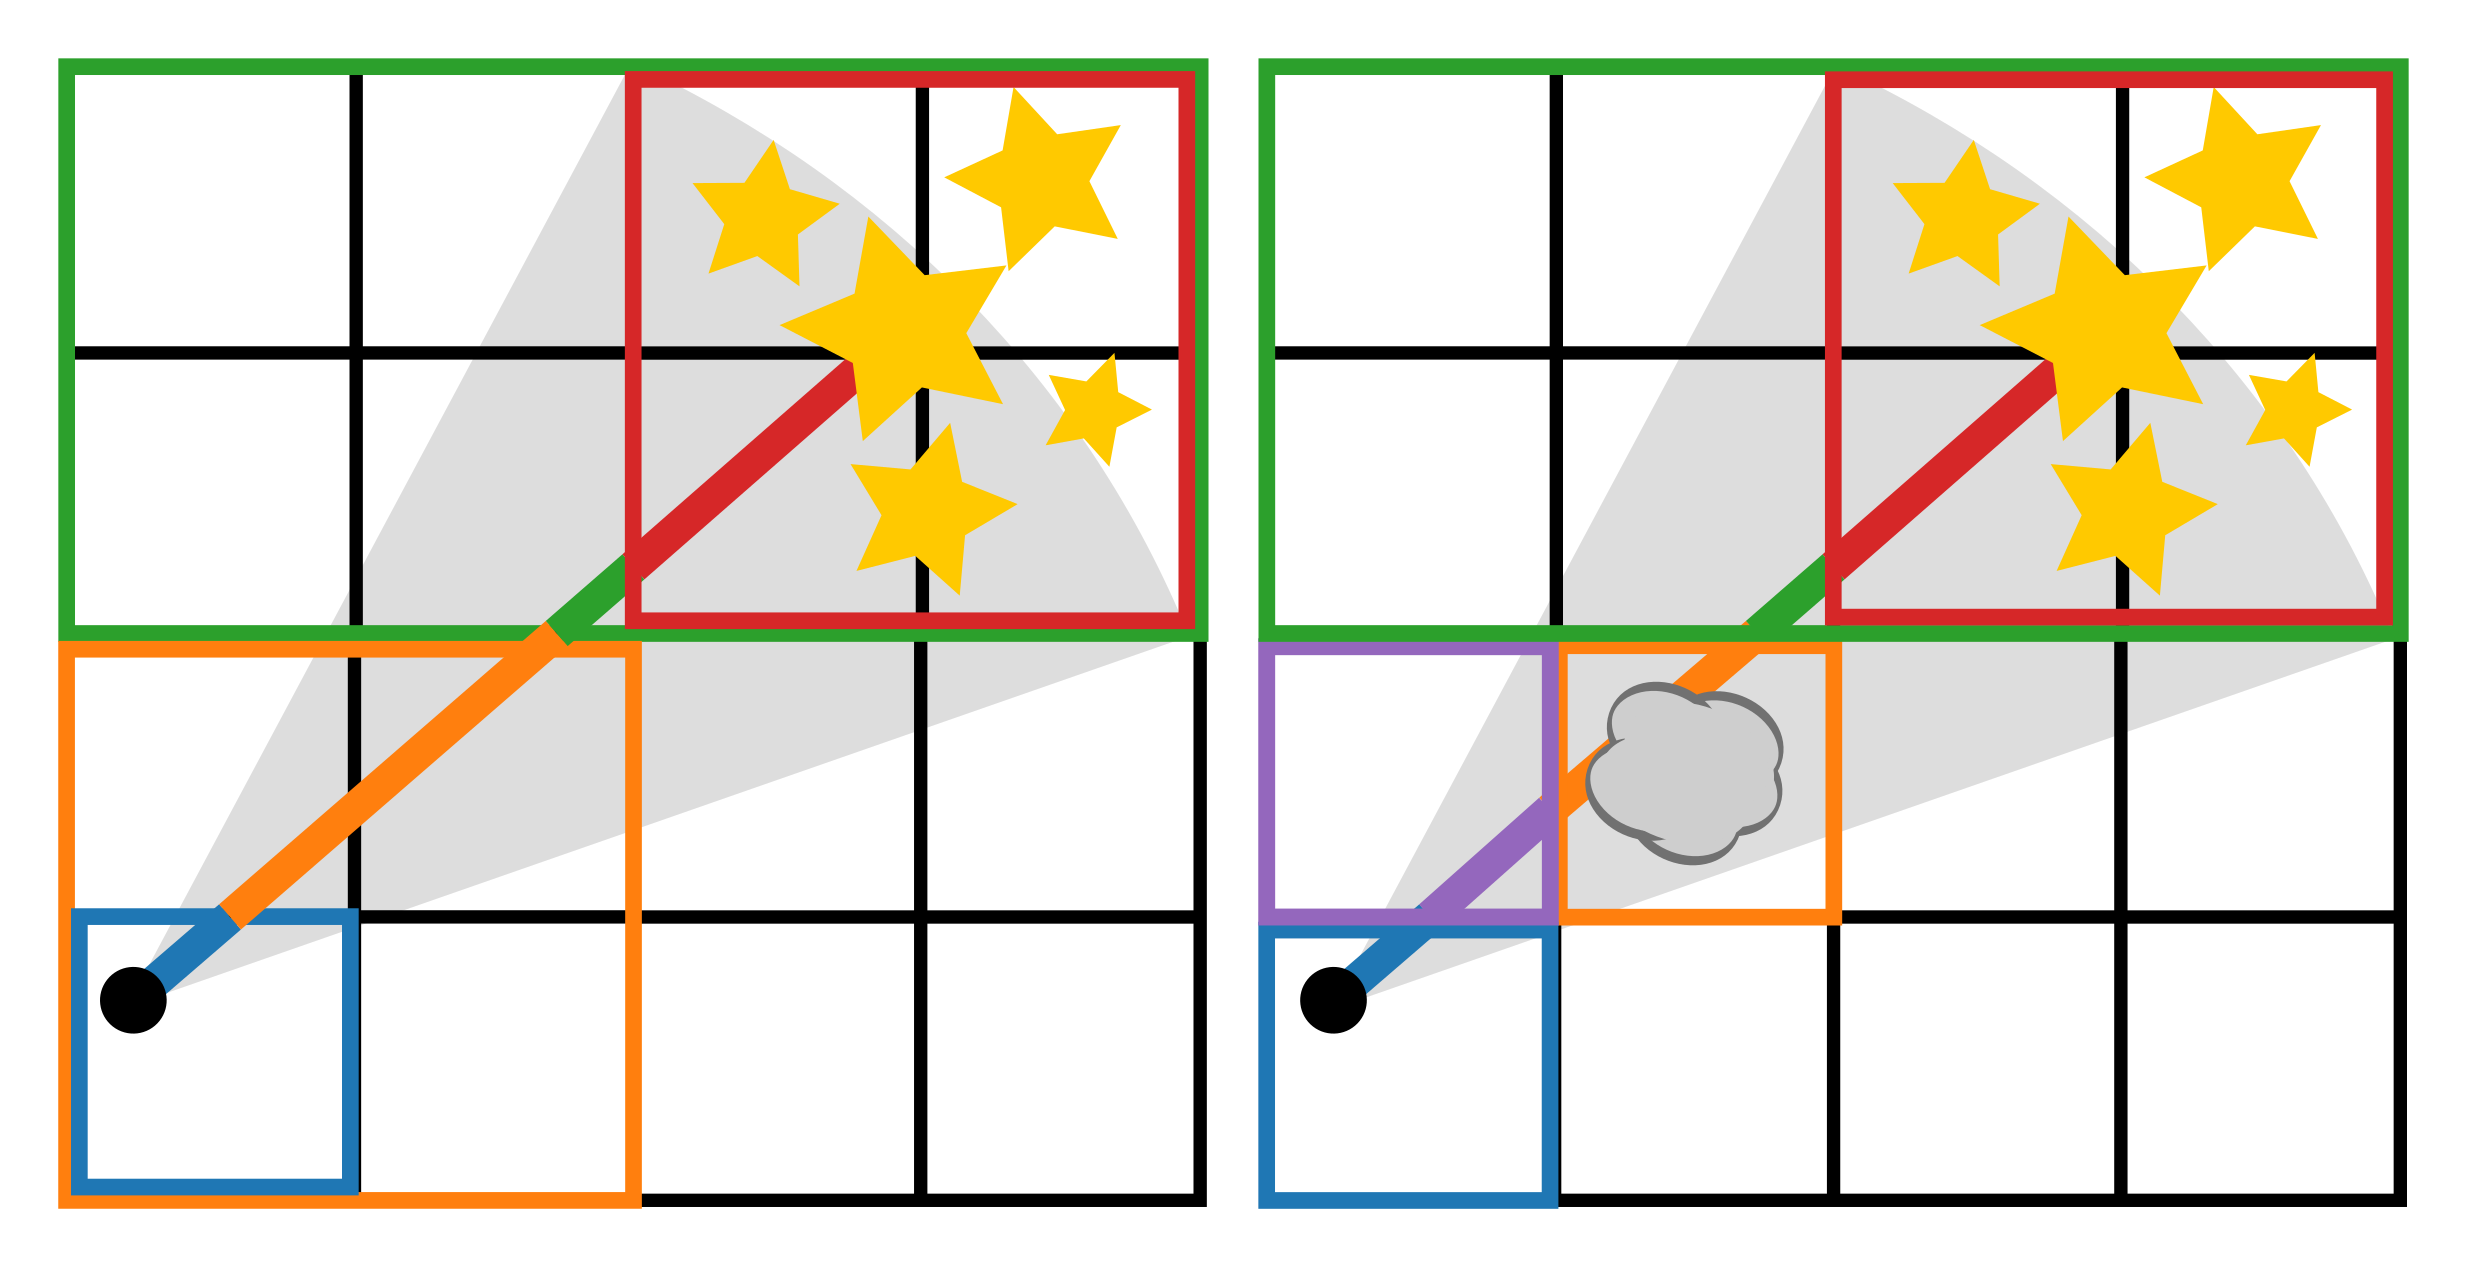
\includegraphics[width=1\linewidth]{Figures/algorithm.png}
\caption{Depiction of the \acro{} algorithm with and without the need for 
refinement (left and right respectively.)}
\label{fig:tree}
\end{figure*}

Difficulty comes in choosing a refinement criteria that is both accurate and 
efficient. Ideally, the criteria should be true when an average optical depth 
in a region may not be accurate to the true distribution, such as a clumpy 
medium where the average opacity is much higher than the ``effective'' opacity
 \citep{hegmanKegel03,varosiDwek99}.

Our choice of refinement criteria is based on optical depth, and is unique to 
the \acro{} algorithm. Consider two rays through a large cell (see figure 
\ref{fig:refine}, note that this description is simplified to 2D).
\begin{figure}
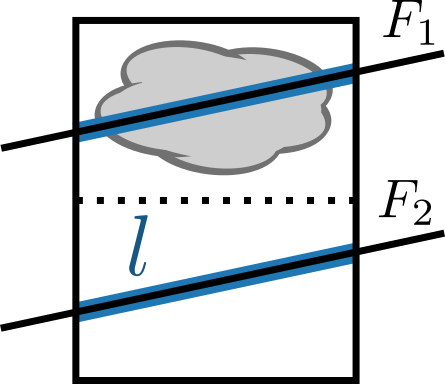
\includegraphics[width=0.45\textwidth]{Figures/refine.png}
\caption{refine.pdf}
\label{fig:refine}
\end{figure}
These rays represent what the case would be if the properties of the children 
were used instead of the parent cell. We can calculate the minimum and maximum 
absorption coefficients $\alpha_{\rm min}$ and $\alpha_{\rm max}$, via their 
average density and opacity values computed during the tree build. This 
multiplied by the intersection $l$, gives us the minimum and maximum optical 
depths, $\tau_{\rm min}$ and $\tau_{\rm max}$. We can then test the following 
refinement criteria
\begin{equation}
\tau_{\rm refine} < \tau_{\rm max} - \tau_{\rm min},
\end{equation}
and refine if it is true. The fractional error in flux for a chosen value of 
$\tau_{\rm refine}$ is 
\begin{equation}
{\rm Fractional Error} = \frac{F_1-F_2}{F_1} \leq 1 - e^{(-\tau_{\rm max} - 
\tau_{\rm min})} < \tau_{\rm refine},
\end{equation}
for small $\tau$, making the refinement criteria a convenient choice of 
parameter for guaranteeing accuracy.  This criteria is conservative, as it 
assumes the worst case difference in optical depth. We suspect there is room 
for improvement in terms of efficiency.

If very high accuracy is required, sub-leaf node refinement is possible. If a 
leaf was reached during refinement and still passes the refinement criteria, 
the individual particles in the leaf can be considered. A ray tracing scheme 
through the cell similar to SPHRay \citep{altayEt08} can be performed. 
The machinery to do this is implemented in \acro{}.

\subsection{Cosmological Background Radiation}
In order to treat cosmological simulations properly we must account for the 
radiation coming from the rest of the universe outside of the simulation 
volume. Most current codes apply a constant UV field to the entire box, 
essentially the lowest order approximation possible. Some specialized codes 
like URCHIN \citep{altayTheuns13} do a reverse ray trace to the edge of the 
box, where the background flux is assumed to be coming from. Others, such as 
TRAPHIC \citep{pawlikSchaye08} allow their ray trace to be periodic. We believe
 that this periodic treatment is problematic for reasons we will explain at the
 end of this subsection. 

Instead, we have implemented a method involving ``background sources''. 
``Background'' particles are distributed in a spiral pattern on the surface of 
a sphere at the very edge of the simulation volume (or at a large distance if 
required) and the number of sources can be varied to match the required angular
 resolution  of the background. Finding the flux at the centre of a sphere of 
sources is a problem akin to Newton's Shell Theorem. However, because the 
intensity does not cancel like force, the solution differs and is as follows:
\begin{equation}\label{eq:cosmofield}
F(r) = \frac{L}{8\pi R} \ln \left(\frac{R+r}{R-r}\right),
\end{equation}
where $L$ is the total luminosity of the emitting shell, $R$ is the radius of 
the sphere and $r$ is the radius the flux is being computed at. The shape of 
the function can be seen if Figure \ref{fig:cosmofield}
\begin{figure}
\label{fig:cosmofield}
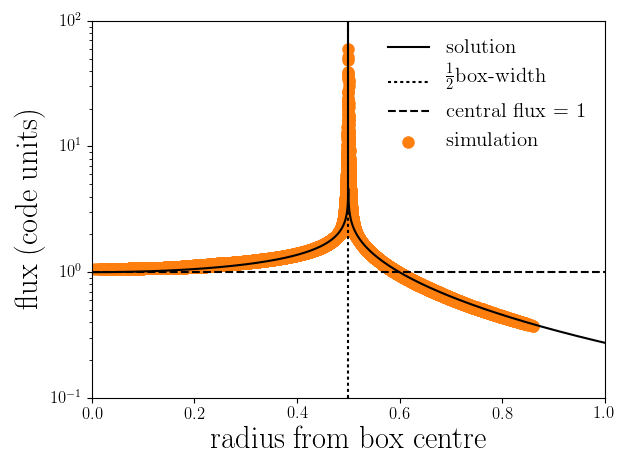
\includegraphics[width=0.5\textwidth]{Figures/cosmofield.png}
\caption{The distribution of flux that particles receive due to the 
cosmological background sources when distributed in a spherical shell on at the
 edge of the simulation box. Note that the value of the flux at the centre can
 be easily scaled by simply scaling $L$, the luminosity of all sources on the 
sphere. The important property is the near constant flux at small radii. In
 this example, we have used 1024 background sources. The number of sources 
determines the width of the peak.}
\end{figure}
where we have plotted the flux as a function of radius for a homogeneous,
optically thin test volume.

We note that due to the logarithm in equation \ref{eq:cosmofield}, the flux is
 nearly constant at small radii. Since most cosmological zoom in simulations 
only consider gas at a fairly small radius, this setup of background sources is
 an acceptable method to provide a cosmological background flux. A benefit of
 this method is that we can use all of the existing machinery described in the 
methods section, and only have to add temporary background star particles as 
the source of the background radiation. This way, there is no need to create 
periodic copies of the simulation volume. **explain <-this here**

\section{CODE TESTS}\label{sec:tests}

\section{DISCUSSION AND CONCLUSION}\label{sec:dandc}

\section*{Acknowledgements}

%%%%%%%%%%%%%%%%%%%%%%%%%%%%%%

%%%%%%%%%% REFERENCES %%%%%%%%%%

\bibliographystyle{mnras}
\bibliography{references}

%%%%%%%%%%%%%%%%%%%%%%%%%%%%%%

%%%%%%%%%% APPENDICES %%%%%%%%%%

\appendix

%%%%%%%%%%%%%%%%%%%%%%%%%%%%%%

\bsp
\label{lastpage}
\end{document}

%%%%%%%%%% FIN %%%%%%%%%%
